\section{Specification and Design}
\label{sec:design}

% ── Mark scheme: 15 marks ─────────────────────────────────────────────────────

\subsection{Architecture Divides Pure Game Logic from Hardware I/O}

The system follows a strict three-tier architecture separating game logic, communication, and presentation.
To ensure that the embedded server remains testable without requiring physical hardware in every unit test, the firmware is split into two distinct layers:
\begin{itemize}
    \item \textbf{Pure Logic Layer (\texttt{game.c}, \texttt{protocol.c})}: Maintains the 9-cell board array, active turn indicator, move validation rules, and ASCII frame parsing. It has zero dependencies on STM32 hardware registers and can be compiled and verified natively on a host PC.
    \item \textbf{Hardware Driver Layer (\texttt{main.c}, \texttt{hardware.c})}: Manages the USART1 peripheral, ring buffers, GPIO push-pull drivers for the status LEDs, and debouncing for the push button.
\end{itemize}

On the host PC, the client is similarly divided between \texttt{serial\_client.py} (which handles raw PySerial frame framing and timeout management) and \texttt{gui.py} (which renders the Tkinter visual window).
Table~\ref{tab:responsibilities} explicitly outlines the ownership of each system responsibility.
The host GUI is entirely ``thin'': it never decides whether a move is legal, never checks for 3-in-a-row, and never advances the turn counter on its own.

\begin{table}[t]
\centering
\caption{System responsibility allocation between client and server.}
\label{tab:responsibilities}
\footnotesize
\begin{tabular}{@{}L{3.5cm}L{1.8cm}L{2.5cm}@{}}
\toprule
Responsibility & Owner & Module \\
\midrule
Board state storage & Server & \texttt{game.c} (\texttt{g\_board}) \\
Turn enforcement & Server & \texttt{game.c} (\texttt{g\_current\_player}) \\
Move legality validation & Server & \texttt{game.c} (\texttt{game\_process\_move}) \\
Win / Draw detection & Server & \texttt{game.c} (\texttt{check\_winner}) \\
Physical status LEDs & Server & \texttt{hardware.c} (PB10, PB11) \\
Hardware reset trigger & Server & \texttt{hardware.c} (PA0 Button) \\
User input forwarding & Client & \texttt{gui.py} \\
Board rendering & Client & \texttt{gui.py} (Tkinter grid) \\
Lifecycle controls (New, Resign, Disconnect) & Client & \texttt{gui.py} \\
Serial link timeouts & Client & \texttt{serial\_client.py} \\
\bottomrule
\end{tabular}
\end{table}

\begin{figure*}[t]
\centering
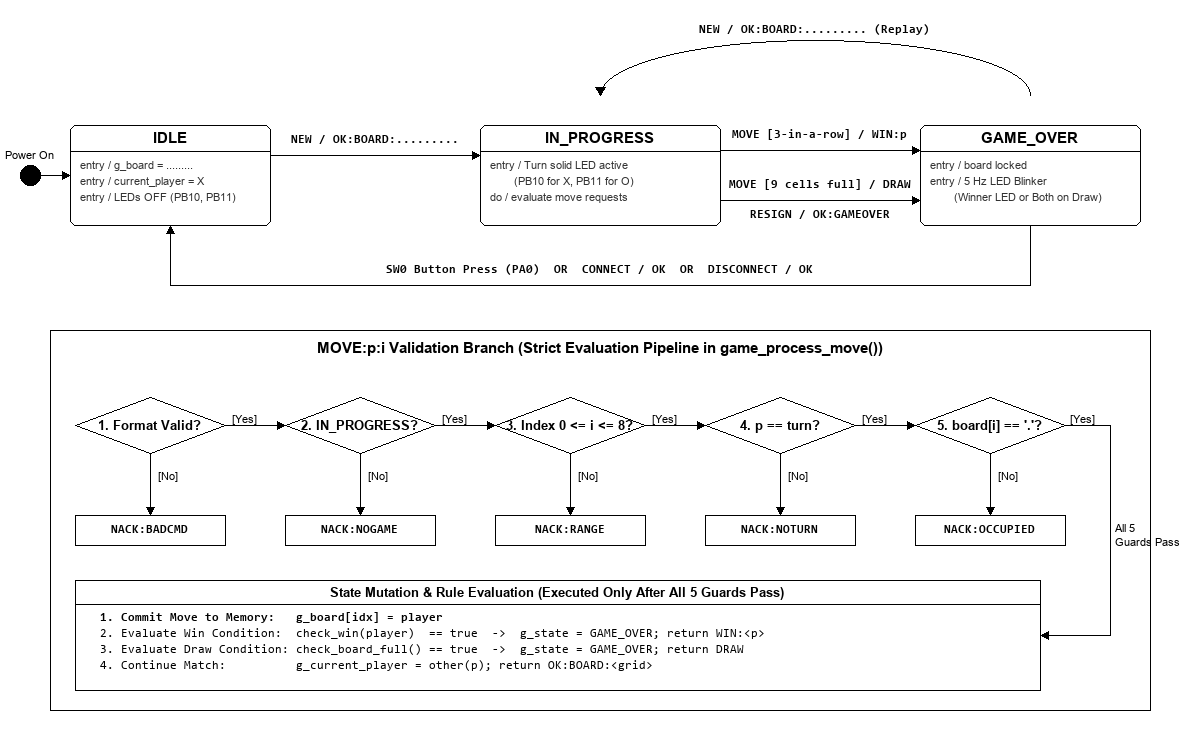
\includegraphics[width=\textwidth]{figures/fsm.png}
\caption{STM32 server Finite State Machine (FSM) showing the three primary states (\texttt{IDLE}, \texttt{IN\_PROGRESS}, and \texttt{GAME\_OVER}), all valid transitions, and the five-stage move-validation pipeline evaluated inside \texttt{game\_process\_move()}.}
\label{fig:fsm}
\end{figure*}

\subsection{The Server Finite State Machine Enforces the Turn and Move Rules}

The server behaviour is governed by a three-state Finite State Machine (FSM) shown in Fig.~\ref{fig:fsm}.
The active state determines which incoming commands are executed and which are rejected with \texttt{NACK:NOGAME}:

\begin{enumerate}
    \item \textbf{\texttt{IDLE}}: Entered upon power-on reset, after an explicit \texttt{CONNECT} or \texttt{DISCONNECT} handshake, or whenever the physical push button (\texttt{SW0}) is pressed. The board contains nine empty dots (\texttt{.........}), the turn defaults to Player~X, and all status LEDs are turned off. Incoming \texttt{MOVE} or \texttt{RESIGN} commands are rejected with \texttt{NACK:NOGAME}. The server transitions to \texttt{IN\_PROGRESS} only when a valid \texttt{NEW} command is received.
    \item \textbf{\texttt{IN\_PROGRESS}}: Indicates an active game. The physical LEDs indicate whose turn it is (Red for Player~X, Green for Player~O). When a \texttt{MOVE:p:i} command arrives, the server executes the move-validation branch before mutating any internal memory.
    \item \textbf{\texttt{GAME\_OVER}}: Entered when three matching marks form a row, column, or diagonal, when all nine cells are occupied without a winner (draw), or when a player submits \texttt{RESIGN}. The board is frozen and no further moves are accepted. The winner's corresponding LED blinks at 5\,Hz (both LEDs blink on a draw). Receiving \texttt{NEW} resets the board and starts a fresh match in \texttt{IN\_PROGRESS}.
\end{enumerate}

\subsubsection{Sequential Gatekeeping Precludes Memory Mutation on Rejected Moves}
As illustrated along the lower pipeline of Fig.~\ref{fig:fsm}, the server checks move validity in five sequential stages inside \texttt{game\_process\_move()}:
\begin{enumerate}
    \item \textbf{Length and Command Syntax}: Frames exceeding 64 bytes or lacking proper colon delimiters return \texttt{NACK:BADCMD}.
    \item \textbf{Active State Check}: If the state is not \texttt{IN\_PROGRESS}, the server returns \texttt{NACK:NOGAME}.
    \item \textbf{Index Range Check}: The cell index string is converted to an integer; if non-numeric or outside the range 0 to 8, the server returns \texttt{NACK:RANGE}.
    \item \textbf{Turn Check}: The player token $p \in \{\texttt{X}, \texttt{O}\}$ is compared against \texttt{g\_current\_player}. If they do not match, the server returns \texttt{NACK:NOTURN}.
    \item \textbf{Occupancy Check}: The target array element \texttt{g\_board[i]} must equal \texttt{'.'}. If already occupied by \texttt{X} or \texttt{O}, the server returns \texttt{NACK:OCCUPIED}.
\end{enumerate}
If any check fails, the validation pipeline terminates immediately with the corresponding NACK, leaving the board array and turn counter strictly unchanged.
Only when all checks pass does the server write the token into the array, evaluate win/draw conditions, alternate the active turn, and reply with the new board string.

\begin{figure}[t]
\centering
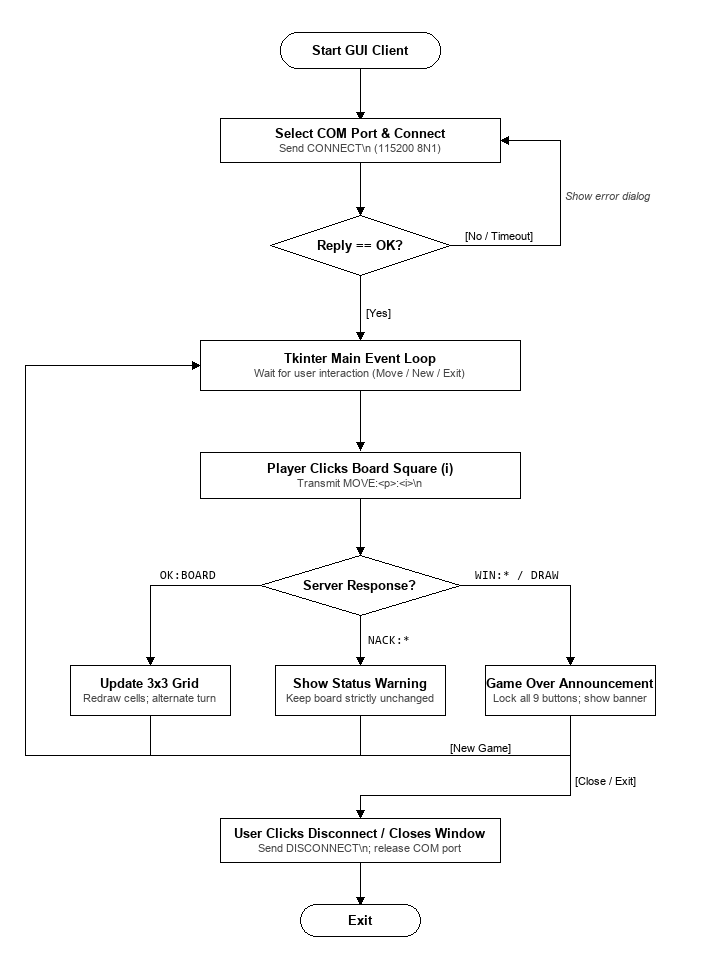
\includegraphics[width=\columnwidth]{figures/gui.png}
\caption{GUI application flowchart showing connection management, event-driven user interaction, and dispatching authoritative responses.}
\label{fig:gui}
\end{figure}

\subsection{The Thin Client Renders State and Never Calculates Legality}

The Python GUI client is designed as a passive display terminal.
Its control flow is detailed in Fig.~\ref{fig:gui}.
Upon startup, the user selects the serial COM port (or connects to the local mock server).
The client transmits \texttt{CONNECT\textbackslash n} and awaits \texttt{OK\textbackslash n}.
To prevent the graphical interface from freezing during serial I/O, the underlying \texttt{serial\_client} module uses a per-read timeout of $1.0\text{ s}$.
If the microcontroller is disconnected or fails to reply within this window, the client catches the timeout exception, displays a non-blocking error dialog, and prompts the user to reconnect.

When a player clicks a board square, the GUI does not mark the square locally.
Instead, it looks up its local assumption of the active player (\texttt{self.current\_player}, initialised to \texttt{X} on \texttt{NEW}) and transmits \texttt{MOVE:p:i\textbackslash n}.
Crucially, the client alternates \texttt{self.current\_player} \emph{only after} the server confirms the move with an authoritative \texttt{OK:BOARD:grid} response.
If the client becomes desynchronized or attempts to send an invalid token, the server's authoritative check (\texttt{player == g\_current\_player}) detects the mismatch and returns \texttt{NACK:NOTURN}, preventing the GUI from overriding the true game state.
The GUI branches on the server's single-line response:
\begin{itemize}
    \item \textbf{\texttt{OK:BOARD:grid}}: The GUI parses the 9-character grid, updates button labels and colors to match the server's array, and advances the visual turn indicator.
    \item \textbf{\texttt{NACK:*}}: The GUI leaves the grid unmodified and displays the error message in the status bar (e.g., ``Move rejected by server: NOTURN'').
    \item \textbf{\texttt{WIN:p} or \texttt{DRAW}}: The GUI locks all nine grid buttons, highlights the winning line, and displays the game over announcement.
\end{itemize}
Beyond move submission, the client provides dedicated controls for session management: a ``New Game'' button transmitting \texttt{NEW}, a ``Resign'' button confirming player forfeiture and transmitting \texttt{RESIGN} (moving the server to \texttt{GAME\_OVER}), and a ``Disconnect'' button that issues \texttt{DISCONNECT} and releases the serial port cleanly.

\subsection{The Board Interfaces via Virtual COM Port, GPIO LEDs, and Button}

\begin{figure}[t]
\centering
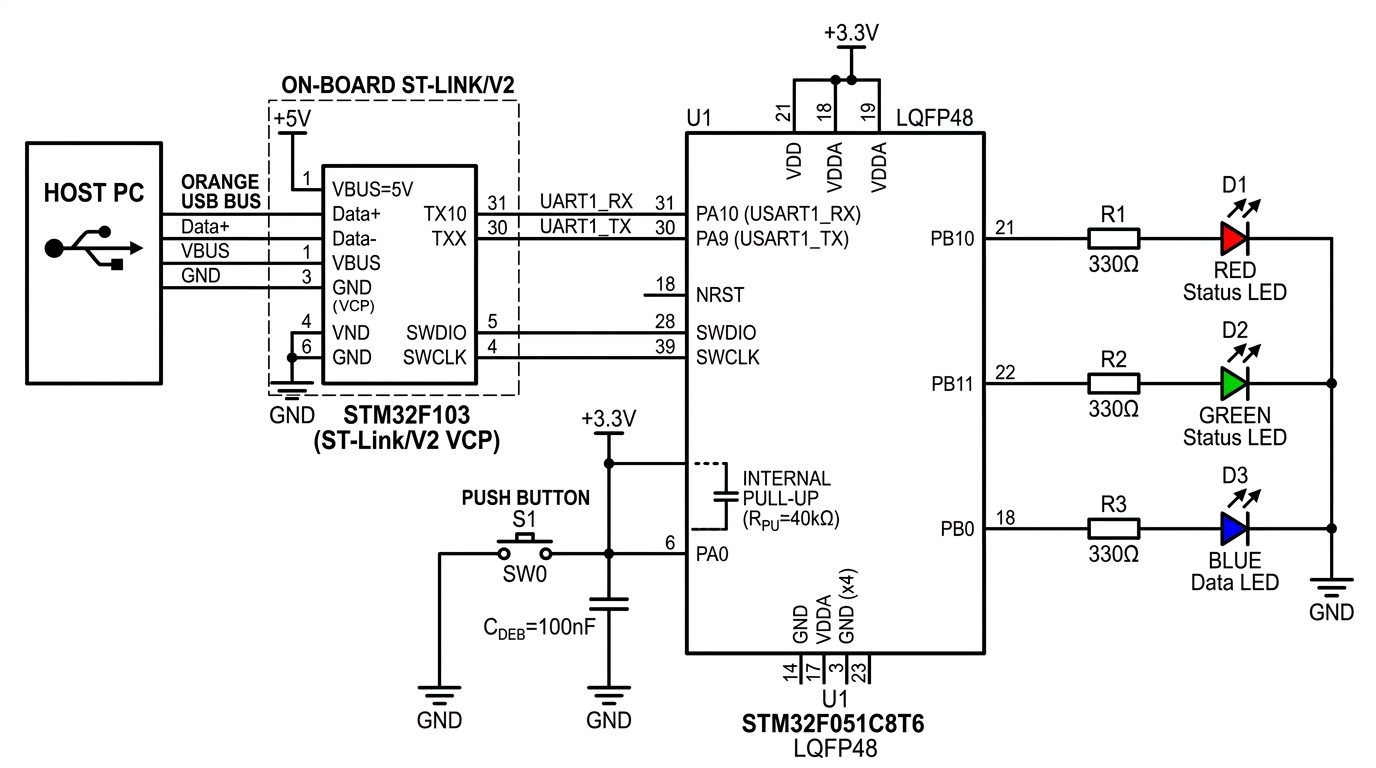
\includegraphics[width=\columnwidth]{figures/circuit.png}
\caption{Hardware circuit diagram showing the STM32F051C8T6 connection to the onboard ST-Link/V2 Virtual COM Port, status LEDs, and reset button.}
\label{fig:circuit}
\end{figure}

The physical circuit implementation is shown in Fig.~\ref{fig:circuit}.
Communication between the host PC and the target microcontroller (U1, an \textbf{STM32F051C8T6} in a 48-pin LQFP package) is routed through the onboard \textbf{ST-Link/V2} interface chip (STM32F103):
\begin{itemize}
    \item \textbf{Serial Link}: The microcontroller's \texttt{PA9} (\texttt{USART1\_TX}) and \texttt{PA10} (\texttt{USART1\_RX}) connect directly to the ST-Link's UART pins, which are exposed over USB as a standard Virtual COM Port operating at 115\,200 baud, 8N1.
    \item \textbf{Status LEDs}: Three low-current LEDs are connected to port B:
    \begin{itemize}
        \item \textbf{Red LED (D1)} on \texttt{PB10}: Indicates Player~X's turn during play, and blinks at 5\,Hz when Player~X wins.
        \item \textbf{Green LED (D2)} on \texttt{PB11}: Indicates Player~O's turn during play, and blinks at 5\,Hz when Player~O wins.
        \item \textbf{Blue Data LED (D3)} on \texttt{PB0}: Toggles on every valid serial byte reception to provide visual link activity feedback.
    \end{itemize}
    Each LED is driven in active-high push-pull mode through a $330\,\Omega$ series current-limiting resistor, drawing approximately $3.9\,\text{mA}$, well within the $25\,\text{mA}$ pin limit.
    \item \textbf{Push Button (SW0)}: Connected to \texttt{PA0}. The pin uses the microcontroller's internal pull-up resistor ($\approx 40\,\text{k}\Omega$) and is pulled to ground (active-low) when pressed. An external $100\,\text{nF}$ capacitor (\(C_{\text{DEB}}\)) and a 50\,ms software accumulator in \texttt{hardware.c} eliminate mechanical contact bounce. Pressing \texttt{SW0} executes \texttt{game\_init()}, resetting the game state to \texttt{IDLE}, restoring an empty board, and extinguishing the status LEDs, while leaving serial protocol framing buffers intact.
\end{itemize}
